\chapter{Background and context}
%\emph{This chapter contains all the information needed to put the thesis into context. It is common to use a revised version of your literature survey for this purpose. It is important to explicitly refer from your text to sources you have used, they will be listed in your bibliography.}

In this chapter we give more background information about the technology stack that is relevant to this thesis. Not all technologies are in use at the client at the moment, but we include them to provide more information about alike technologies or new technologies that we could use. We start with containers and container orchestration platforms which form the basics of running workloads. Next we explore the different virtual networks technologies with \gls{cni}.

\section{Containers}
\subsection{Docker}
\subsection{Kubernetes}
\subsection{DC/OS}

\section{CNI}
\todo[inline]{CNI and/vs libnetwork}

\subsection{Standard plugins}
There are a set of standard provided plugins\cite{cni_plugin} that allow for basic operations like creating network interfaces and IP address allocation. Different kind of interfaces can be created such as bridges, loopback interfaces and vlans. IP addresses can be either requested from a \gls{dhcp} server or maintained by a local database of allocated IPs. Other plugin providers can provide their own implementations of assigning IP address to containers.

\subsection{Project Calico}
Project Calico uses a pure Layer 3 approach to enable virtual networking between container workloads. As opposed to traditional solutions which mostly use overlay networks. Overlay networks have the extra burden of en- and decapitation packages between workloads when the traffic crosses different machines. Without this Calico is able to save \gls{cpu} cycles and makes it easier to understand packets on the wire. Performance tests\cite{dzone, dataplane, chunqi} show that Calico is able to achieve nearly identical throughput to direct connect workloads. Overlay networks, and other techniques such as Weave\cite{weave} are not able to reach this throughput.

Instead of using a vSwitch, Calico uses a vRouter to route traffic between containers. This vRouter uses the Layer 3 forwarding technique found in the Linux kernel. A local agent, called Felix, programs the routes from the containers to the host in the node's route table. Furthermore, a \gls{bird} is running on every node to advertise routes to containers on other nodes in the cluster. Figure~\ref{fig:hops} shows the hops made between two different containers or workloads. State information is exchanged using \gls{bgp} route reflectors.

By default all containers can talk to each other in a Calico network. Mostly operators want to separate traffic between different tenants of the compute cluster, this can be done by assigning policies. A policy is translated to a rule in iptables\cite{iptables} on the host, leveraging the default Linux firewall. This can even be extended to specific rules for different workloads within a tenancy. The policies are shared using a distributed key-value store called etcd\cite{etcd}, as can be seen in Figure~\ref{fig:calico-arc}.

\begin{figure}
    \centering
    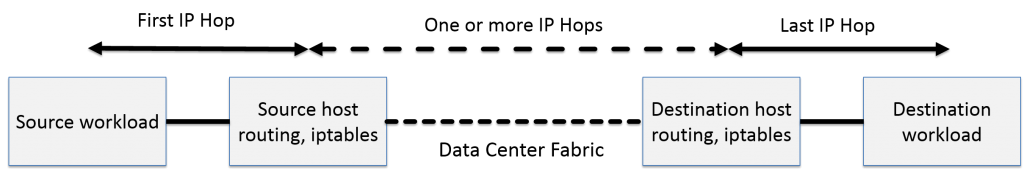
\includegraphics[scale=0.35]{images/calico-hops}
    \caption{IP connectivity in Calico\cite{calico_learn}}
    \label{fig:hops}
\end{figure}

\begin{figure}
    \centering
    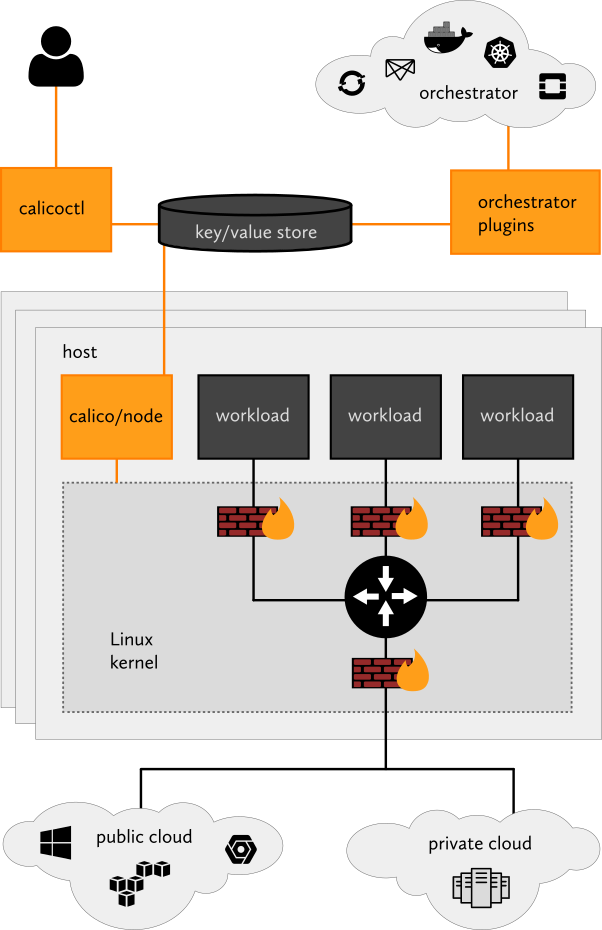
\includegraphics[width=0.4\columnwidth]{images/calico-arch}
    \caption{Project Calico component overview \cite{calico_about}}
    \label{fig:calico-arc}
\end{figure}

\subsection{Cilium}
A plugin that also takes a whole different approach is Cilium\cite{cilium} where they allow for \gls{api} aware security policies. Instead of only operating at the network level with host and port based firewall rules, Cilium allows filtering of different protocols like \gls{http}, \gls{grpc}\cite{grpc} and Kafka\cite{kafka}. They do this by leveraging a new Linux kernel technology called \gls{bpf}\cite{mccanne1993bsd, cilium_bpf} by dynamically inserting \gls{bpf} bytecode into the Linux kernel, as can be seen in Figure~\ref{fig:cilium-arch}. 

This \gls{cni} plugin creates \gls{bpf} programs in the Linux kernel that control the network access. The \gls{bpf} programs are \gls{jit} compiled to \gls{cpu} instructions to allow for native execution performance. You can do a lot of different things with this technology; simply monitoring the packets, redirecting packets and blocking packets. Only recent versions of the Linux kernel have \gls{bpf} capabilities, version 4.8.0 or newer is required. 

\begin{figure}
    \centering
    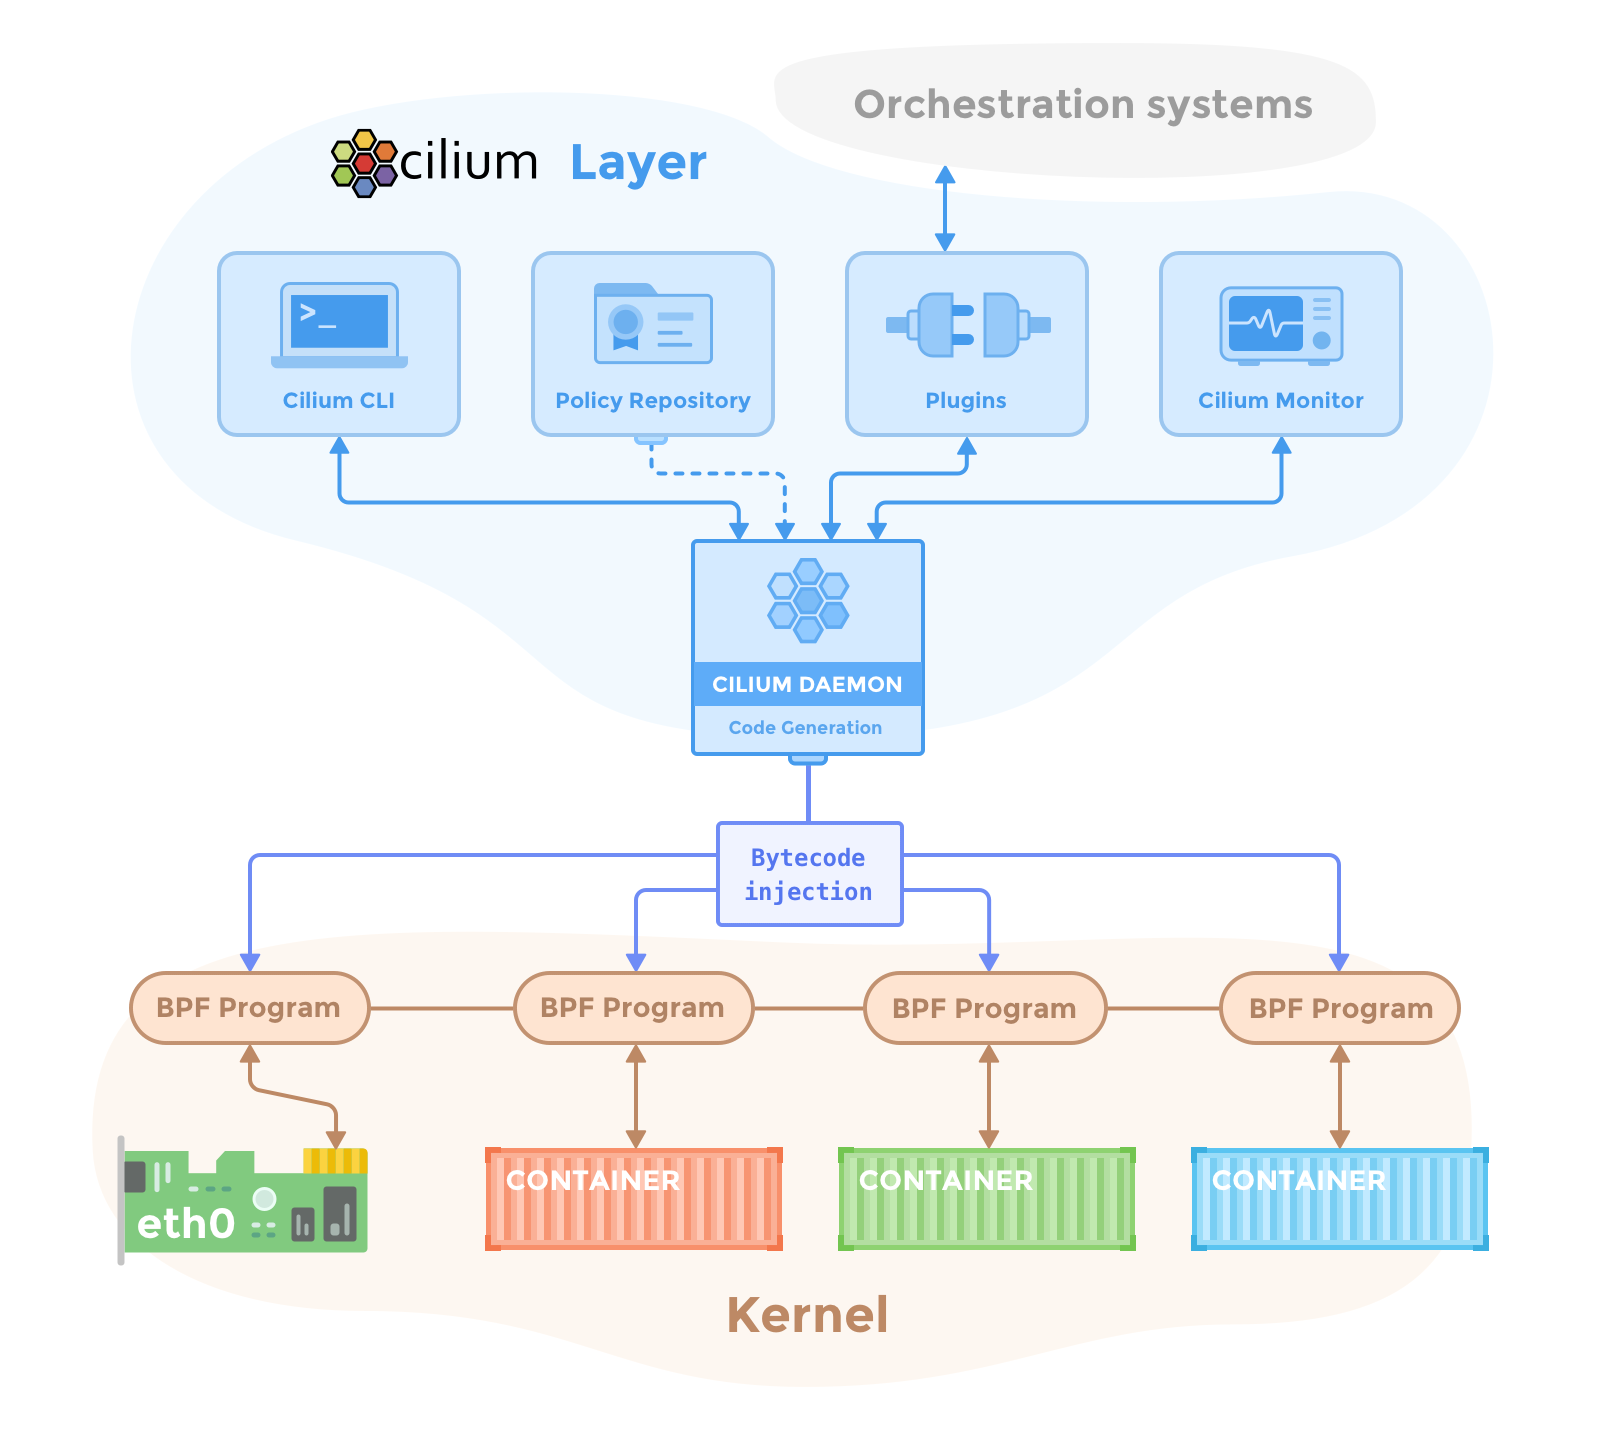
\includegraphics[width=0.7\columnwidth]{images/cilium-arch}
    \caption{Cilium component overview \cite{cilium_concepts}}
    \label{fig:cilium-arch}
\end{figure}
